\documentclass[CJK]{beamer}
%\usepackage{CJKutf8}
\usepackage{beamerthemesplit}
\usepackage{}
%\usetheme{Frankfurt}
%\usetheme{CambridgeUS}
%\usecolortheme{beaver}
%\usetheme{AnnArbor}
\usetheme{Dresden}
%\usebeamercolor{beetle}
\usepackage{xeCJK}
\setCJKmainfont{AR PL KaitiM GB}
%\useoutertheme{miniframes}
\usepackage{amsmath}
\usepackage{graphicx}
\usepackage{float} 
\usepackage{subfigure}
\usepackage{amssymb}
\usepackage{graphicx}
\usepackage{eufrak}
\usepackage{color}
\usepackage{array}
\usepackage{slashed}
\usepackage{simplewick}
\usepackage{tikz}
\usepackage{tcolorbox}
\usepackage[T1]{fontenc}
\graphicspath{{../figures/}}

%%figures
\def\lfig#1#2{\includegraphics[width=#1 in]{#2}}
\def\addfig#1#2{\begin{center}\includegraphics[width=#1 in]{#2}\end{center}}
\def\wulian{
\includegraphics[width=0.18in]{emoji_wulian.jpg}}
\def\bigwulian{
\includegraphics[width=0.35in]{emoji_wulian.jpg}}
\def\bye{
\includegraphics[width=0.18in]{emoji_bye.jpg}}
\def\bigbye{
\includegraphics[width=0.35in]{emoji_bye.jpg}}
\def\huaixiao{
\includegraphics[width=0.18in]{emoji_huaixiao.jpg}}
\def\bighuaixiao{
\includegraphics[width=0.35in]{emoji_huaixiao.jpg}}
\def\jianxiao{
\includegraphics[width=0.18in]{emoji_jianxiao.jpg}}
\def\bigjianxiao{
\includegraphics[width=0.35in]{emoji_jianxiao.jpg}}
%% colors
\def\blacktext#1{{\color{black}#1}}
\def\bluetext#1{{\color{blue}#1}}
\def\redtext#1{{\color{red}#1}}
\def\darkbluetext#1{{\color[rgb]{0,0.2,0.6}#1}}
\def\skybluetext#1{{\color[rgb]{0.2,0.7,1.}#1}}
\def\cyantext#1{{\color[rgb]{0.,0.5,0.5}#1}}
\def\greentext#1{{\color[rgb]{0,0.7,0.1}#1}}
\def\darkgray{\color[rgb]{0.2,0.2,0.2}}
\def\lightgray{\color[rgb]{0.6,0.6,0.6}}
\def\gray{\color[rgb]{0.4,0.4,0.4}}
\def\blue{\color{blue}}
\def\red{\color{red}}
\def\green{\color{green}}
\def\darkgreen{\color[rgb]{0,0.4,0.1}}
\def\darkblue{\color[rgb]{0,0.2,0.6}}
\def\skyblue{\color[rgb]{0.2,0.7,1.}}
%%control
\def\be{\begin{equation}}
\def\ee{\nonumber\end{equation}}
\def\bea{\begin{eqnarray*}}
\def\eea{\nonumber\end{eqnarray*}}
\def\bch{}
\def\ech{}
\def\bitem{\begin{itemize}}
\def\eitem{\end{itemize}}
\def\bcenter{\begin{center}}
\def\ecenter{\end{center}}
\def\bex{\begin{minipage}{0.2\textwidth}
\includegraphics[width=0.6in]{jugelizi.png}\end{minipage}\begin{minipage}{0.76\textwidth}}
\def\eex{\end{minipage}}
\def\chtitle#1{\frametitle{\bch#1\ech}}
\def\bmat#1{\left(\begin{array}{#1}}
\def\emat{\end{array}\right)}
\def\bcase#1{\left\{\begin{array}{#1}}
\def\ecase{\end{array}\right.}
\def\bmini#1{\begin{minipage}{#1\textwidth}}
\def\emini{\end{minipage}}
\def\tbox#1{\begin{tcolorbox}#1\end{tcolorbox}}
\def\pfrac#1#2#3{\left(\frac{\partial #1}{\partial #2}\right)_{#3}}
%%symbols
\def\bropt{\,(\ \ \ )}
\def\sone{$\star$}
\def\stwo{$\star\star$}
\def\sthree{$\star\star\star$}
\def\sfour{$\star\star\star\star$}
\def\sfive{$\star\star\star\star\star$}
\def\rint{{\int_\leftrightarrow}}
\def\roint{{\oint_\leftrightarrow}}
\def\stdHf{{\textit{\r H}_f}}
\def\deltaH{{\Delta \textit{\r H}}}
\def\ii{{\dot{\imath}}}
\def\skipline{{\vskip0.1in}}
\def\skiplines{{\vskip0.2in}}
\def\lagr{{\mathcal{L}}}
\def\hamil{{\mathcal{H}}}
\def\vecv{{\mathbf{v}}}
\def\vecx{{\mathbf{x}}}
\def\vecy{{\mathbf{y}}}
\def\veck{{\mathbf{k}}}
\def\vecp{{\mathbf{p}}}
\def\vecn{{\mathbf{n}}}
\def\vecA{{\mathbf{A}}}
\def\vecP{{\mathbf{P}}}
\def\vecsigma{{\mathbf{\sigma}}}
\def\hatJn{{\hat{J_\vecn}}}
\def\hatJx{{\hat{J_x}}}
\def\hatJy{{\hat{J_y}}}
\def\hatJz{{\hat{J_z}}}
\def\hatj#1{\hat{J_{#1}}}
\def\hatphi{{\hat{\phi}}}
\def\hatq{{\hat{q}}}
\def\hatpi{{\hat{\pi}}}
\def\vel{\upsilon}
\def\Dint{{\mathcal{D}}}
\def\adag{{\hat{a}^\dagger}}
\def\bdag{{\hat{b}^\dagger}}
\def\cdag{{\hat{c}^\dagger}}
\def\ddag{{\hat{d}^\dagger}}
\def\hata{{\hat{a}}}
\def\hatb{{\hat{b}}}
\def\hatc{{\hat{c}}}
\def\hatd{{\hat{d}}}
\def\hatN{{\hat{N}}}
\def\hatH{{\hat{H}}}
\def\hatp{{\hat{p}}}
\def\Fup{{F^{\mu\nu}}}
\def\Fdown{{F_{\mu\nu}}}
\def\newl{\nonumber \\}
\def\vece{\mathrm{e}}
\def\calM{{\mathcal{M}}}
\def\calT{{\mathcal{T}}}
\def\calR{{\mathcal{R}}}
\def\barpsi{\bar{\psi}}
\def\baru{\bar{u}}
\def\barv{\bar{\upsilon}}
\def\qeq{\stackrel{?}{=}}
\def\torder#1{\mathcal{T}\left(#1\right)}
\def\rorder#1{\mathcal{R}\left(#1\right)}
\def\contr#1#2{\contraction{}{#1}{}{#2}#1#2}
\def\trof#1{\mathrm{Tr}\left(#1\right)}
\def\trace{\mathrm{Tr}}
\def\comm#1{\ \ \ \left(\mathrm{used}\ #1\right)}
\def\tcomm#1{\ \ \ (\text{#1})}
\def\slp{\slashed{p}}
\def\slk{\slashed{k}}
\def\calp{{\mathfrak{p}}}
\def\veccalp{\mathbf{\mathfrak{p}}}
\def\Tthree{T_{\tiny \textcircled{3}}}
\def\pthree{p_{\tiny \textcircled{3}}}
\def\dbar{{\,\mathchar'26\mkern-12mu d}}
\def\erf{\mathrm{erf}}
\def\const{\mathrm{constant}}
\def\pheat{\pfrac p{\ln T}V}
\def\vheat{\pfrac V{\ln T}p}
%%units
\def\fdeg{{^\circ \mathrm{F}}}
\def\cdeg{^\circ \mathrm{C}}
\def\atm{\,\mathrm{atm}}
\def\angstrom{\,\text{\AA}}
\def\SIL{\,\mathrm{L}}
\def\SIkm{\,\mathrm{km}}
\def\SIyr{\,\mathrm{yr}}
\def\SIGyr{\,\mathrm{Gyr}}
\def\SIV{\,\mathrm{V}}
\def\SImV{\,\mathrm{mV}}
\def\SIeV{\,\mathrm{eV}}
\def\SIkeV{\,\mathrm{keV}}
\def\SIMeV{\,\mathrm{MeV}}
\def\SIGeV{\,\mathrm{GeV}}
\def\SIcal{\,\mathrm{cal}}
\def\SIkcal{\,\mathrm{kcal}}
\def\SImol{\,\mathrm{mol}}
\def\SIN{\,\mathrm{N}}
\def\SIHz{\,\mathrm{Hz}}
\def\SIm{\,\mathrm{m}}
\def\SIcm{\,\mathrm{cm}}
\def\SIfm{\,\mathrm{fm}}
\def\SImm{\,\mathrm{mm}}
\def\SInm{\,\mathrm{nm}}
\def\SImum{\,\mathrm{\mu m}}
\def\SIJ{\,\mathrm{J}}
\def\SIW{\,\mathrm{W}}
\def\SIkJ{\,\mathrm{kJ}}
\def\SIs{\,\mathrm{s}}
\def\SIkg{\,\mathrm{kg}}
\def\SIg{\,\mathrm{g}}
\def\SIK{\,\mathrm{K}}
\def\SImmHg{\,\mathrm{mmHg}}
\def\SIPa{\,\mathrm{Pa}}
\def\secpage#1#2{\begin{frame}\bch\bcenter{\bf \Huge #1} \skipline \tbox{\bcenter #2\ecenter}\ecenter\ech\end{frame}}

\usepackage{amssymb}
\newcommand{\field}{\mathscr{F}}

\newcommand{\reals}{\mathbb{R}}
\newcommand{\complexs}{\mathbb{C}}
\newcommand{\ints}{\mathbb{Z}}
%\newcommand{\dim}{\mathrm{dim\ }}
\newcommand{\diag}{\mathrm{diag \ }}
\newcommand{\up}{\uparrow}
\newcommand{\down}{\downarrow}
\newcommand{\su}{\mathfrak{su}}
\newcommand{\so}{\mathfrak{so}}
\newcommand{\tr}{\mathrm{tr\ }}
\newcommand{\card}{\mathrm{card \ }}

\newtheorem{thm}{定理}[section]
\newtheorem{axm}{公理}[section]
\newtheorem{dfn}{定义}[section]

%\cpic{<尺寸>}{<文件名>}}用于生成居中的图片。
\newcommand{\cpic}[2]{
\begin{center}
\includegraphics[scale=#1]{#2}
\end{center}
}

%\cpicn{<尺寸>}{<文件名>}{<注释>}用于生成居中且带有注释的图片,其label为图片名。
\newcommand{\cpicn}[3]
{
\begin{figure}[h!]
\cpic{#1}{#2}
\caption{#3\label{#2}}
\end{figure}
}

\title{AQM Talk 9 Phonons}
  \author{}
  \date{}


\begin{document}

\begin{frame}
 
\begin{center}
\begin{Large}
  \bch
  \begin{center}

\includegraphics[width = 1.5in]{whopper}
\end{center}

{\bf A}pplication of {\bf Q}uantum {\bf M}echanics

{\vskip 0.1in}

Talk 9-Phonons

\ech
\end{Large}
\end{center}


\vskip 0.1in
\begin{center}
Haoting Xu
\vskip 0.1in
xuht9@mail2.sysu.edu.cn
\vskip 0.1in
{\tiny \url{https://github.com/HaotingXu/seminar_lec/phonons} }\\
\end{center}


\end{frame}
\begin{frame}\frametitle{\bch内容提要\ech}
  \bch
  \begin{enumerate}
  \item 声音在固体中的传播--经典图像
  \item 原子振动对于能带的影响
  \item 波动方程量子化
  \item 场量子化
    \end{enumerate}
  \begin{center}
    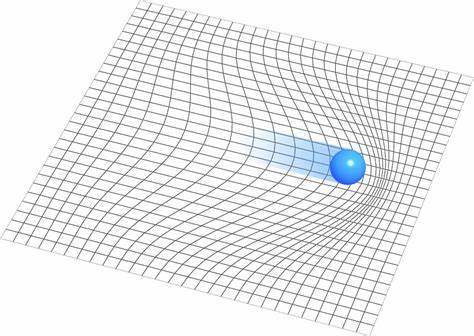
\includegraphics[width = 1.2in]{phonon}
  \end{center}
  \ech
\end{frame}
\section{Classical Phonons}
\begin{frame}\frametitle{\bch 一维全同经典声子\ech}
  \bch
  我们先研究一个最简单的情况,$N$个小球通过“弹簧”链接,并被限制在一条线上运动。平衡位置间距为$a$。
  \cpic{0.25}{monotonic}
  记第$n$个小球的位置为$x_n$,平衡位置则为$x_n = na$,我们只考虑相邻原子的相互作用,将相互作用势能展开到二阶项
  \be
  V = \sum_n V(x_n-x_{n-1}) \simeq \sum_n \frac{\lambda}{2} (x_n - x_{n-1}-a)^2
  \ee
  如果记$u_n(t) = x_n(t) -na$,则系统的哈密顿量为
  \be
  H = \sum_n \frac{p_n^2}{2m}+\frac{\lambda}{2}\sum_n (u_n - u_{n-1})^2
  \ee
  \ech
\end{frame}
\begin{frame}\frametitle{\bch求解运动方程\ech}
  \bch
  由哈密顿正则方程
  \be
  \dot{p}_n = -\frac{\partial H}{\partial q_n}
  \ee
  得到运动方程
  \be
  m\ddot{u_n} = -\lambda (2u_n - u_{n-1} - u_{n+1})
  \ee
  上述运动方程可以使用离散傅里叶变换快速求解,离散傅里叶变换即将数列$u_n$分解为$e^{ikna}$的线性组合,即$u_n = \sum_k a_k e^{ikan}$,在这里我们加入周期性边界条件,我们认为第1个原子和第$N$个原子在无穷远处相连,即$u_{1} = u_{N+1}$,如果引入了这样的边界条件,得到$k$的限制为
  \be
  k = \frac{2\pi}{Na}l,\, l = -\frac{N}{2},\cdots, \frac{N}{2}
  \ee
  $k$的取值为$[-\frac{\pi}{a},\frac{\pi}{a})$,这被称作第一个布里渊区。
    \ech
\end{frame}
\begin{frame}\frametitle{\bch离散傅里叶变换\ech}
  \bch
  根据公式
  \be
  \sum_k e^{ika(m-n)} = N\delta_{mn},\, \sum_n e^{ina(k-k^{\prime})} = N\delta_{kk^{\prime}}
  \ee
  得到离散傅里叶变换的表达式
  \be
  a_k = \frac{1}{N}\sum_n u_ne^{-ikan}
  \ee
  显然,如果$u_n$的傅里叶变换是$a_k$,则$u_{n+d}$的傅里叶变换是$a_ke^{ikda}$。对上面的运动方程做离散傅里叶变换,得到
  \be
  m\ddot{a}_k = -\lambda (2-e^{ika} - e^{-ika})a_k
  \ee
  进而假设$a_k = e^{-i\omega t}$得到色散关系
  \be
  \omega = 2\sqrt{\frac{\lambda}{m}}|\sin(\frac{ka}{2})|
  \ee
  \ech
\end{frame}
\begin{frame}\frametitle{\bch 固体中的声速\ech}
  \bch
  在第一个布里渊区将色散关系画出,如下图
  \cpic{0.3}{mono_dispersion}
  当$k$很小时,求得固体中的声速为
  \be
  c_s = \frac{d\omega}{dk} \simeq \sqrt{\frac{\lambda}{m}}a
  \ee
  \ech
\end{frame}
\begin{frame}\frametitle{\bch双原子链 \ech}
  \bch
  我们更进一步,将全同原子换成两个不同质量的原子交替出现,如下图所示
  \cpic{0.25}{diatomic}
  这时运动方程变为
  \bea
  m\ddot{u}_{2n} &=& -\lambda (2u_{2n} - u_{2n-1} - u_{2n+1})  \\
  M\ddot{u}_{2n+1} &=& -\lambda (2u_{2n+1} - u_{2n} - u_{2n+2})
  \eea
  这时由于双原子出现的周期为$2a$,故作傅里叶变换时,应当将$a$换成$2a$,相应的布里渊区缩小一倍。对上面的方程进行离散傅里叶变换,设奇数项的傅里叶变换为$b_{2n-1}$,偶数项的傅里叶变换为$a_{2n}$,则有
  \bea
  m\ddot{a}_{2n}&=&-\lambda (2a_{2n} - b_{2n+1}(1+e^{-2ika}))\\
  M\ddot{b}_{2n+1}&=& -\lambda (2b_{2n+1} - a_{2n}(1+e^{2ika}))
  \eea
  \ech
\end{frame}
\begin{frame}\frametitle{\bch色散关系\ech}
  \bch
  如果假设$a_{2n} = A e^{-i\omega t},\, b_{2n+1} = B e^{-i\omega t}$则有
  \be
  \omega^2 
  \begin{pmatrix}
    m & 0\\ 0 & M\\
  \end{pmatrix}
    \begin{pmatrix}
      A\\B\\
    \end{pmatrix}
    = \lambda 
    \begin{pmatrix}
      2& -(1+e^{-2ika})\\ -(1+e^{2ika}) & 2\\
    \end{pmatrix}\begin{pmatrix}A\\B\\\end{pmatrix}
        \ee
        若要方程有非零解,则要求
        \be
        \mathrm{det}
        \begin{pmatrix}
          2\lambda - m\omega^2 & -\lambda(1+e^{-2ika}) \\ -\lambda(1+e^{2ika}) & 2\lambda - M\omega^2\\
        \end{pmatrix}
        =0
        \ee
        解出色散关系
          \be
          \omega_{\pm}^2 = \frac{\lambda}{Mm}\left[m+M\pm \sqrt{(m-M)^2+4Mm\cos^2(ka)}\right]
          \ee
  \ech
\end{frame}
\begin{frame}\frametitle{\bch色散关系\ech}
  \bch
  将上面的色散关系画图
  \cpic{0.3}{dia_dispersion}
  其中上面的分支(对应于$\omega_{+}$)叫做光学分支,下面的分支(对应于$\omega_-$)叫做声学分支。下面来解释这两个名词。
  \ech
\end{frame}
\begin{frame}\frametitle{\bch声学分支与光学分支\ech}
  \bch
  我们考虑$k\rightarrow 0$的情况,这时,上面的关系为
  \be
  \begin{pmatrix}
  2\lambda - m\omega^2 & -2\lambda \\ -2\lambda & 2\lambda - M\omega^2\\
  \end{pmatrix}
  \begin{pmatrix}
    A\\B\\
  \end{pmatrix}
  =0
  \ee
  求解本征态,当$\omega$分别为$\omega_-^2 = 0,\,\omega_+^2 = 2\lambda(1/M+1/m)$时
  \be
 \begin{pmatrix}
    A\\B\\
 \end{pmatrix}
 =\begin{pmatrix}
    1\\1\\
  \end{pmatrix}
 ,\,
 \begin{pmatrix}
    A\\B\\
 \end{pmatrix}
 =\begin{pmatrix}
    M\\-m\\
 \end{pmatrix}
 \ee
 可见,在声学分支相邻两个原子振动同相位,在光学分支相邻两个原子振动相位恰好相反。
 \ech
\end{frame}
\begin{frame}\frametitle{\bch声学分支与光学分支\ech}
  \bch
  因此声学分支意味着振动是同相位的,就像声音在固体中传播。在光学分支,相邻两个原子振动反相,在晶体中,相邻两个原子一般电荷相反(如$\mathrm{NaCl}$晶体),反相意味着每两个原子会靠的很近,形成电偶极子,电偶极距的大小会有一个角频率$\omega_+$的振动,这意味着这些小电偶极子可以吸收或发射光子,因此称为光学分支。在实验中确实观察到了这些特点,下图是实验测得的$\mathrm{NaCl}$晶体的色散曲线
  \cpic{0.3}{nacl}
  \ech
\end{frame}
\begin{frame}\frametitle{\bch Peierls跃迁 \ech}
  \bch
  现在我们知道了原子如何振动,我们现在考虑原子振动对电子的价带结构的影响。如果原子不动,我们解出过电子的色散关系,由于周期势的微扰,使得布里渊区分界点附近的色散曲线产生分裂。但是现在由于两个原子不停振动,势能周期减半,布里渊区从$k\in [-\frac{\pi}{a},\frac{\pi}{a}]$变为$k\in [-\frac{\pi}{2a},\frac{\pi}{2a}]$,所以电子的色散曲线如下图所示变化
  \cpic{0.2}{distortion}
  \ech
\end{frame}
\begin{frame}\frametitle{\bch能带断裂后的色散曲线\ech}
  \bch
  电子的哈密顿量为
  \be
  H = \frac{p^2}{2m}+V(x)
  \ee
  其中$V(x)$为周期势。在第二章,我们用微扰理论计算了能带的分裂,即取两个本征态为$|k\rangle,\,|-k\rangle$做简并微扰,即计算矩阵元
  \be
  \begin{pmatrix}
    \langle k|V|k\rangle & \langle -k|V|k\rangle\\
    \langle k|V|-k\rangle & \langle -k|V|-k \rangle\\
  \end{pmatrix}
  \ee
  其中对角元大部分都为0,只有当$k\simeq \frac{\pi}{a}$时才有对角项,所以我们解出了能带的断裂
  \be
  E = \frac{\hbar^2 k^2}{2m}+V_0 \pm V_1
  \ee
  现在我们要求解在$k = \pm \frac{\pi}{a}$附近,断裂后的能量本征值的近似$E_{\pm}(k)$。
  \ech
\end{frame}
\begin{frame}\frametitle{\bch能带断裂后的色散曲线\ech}
  \bch
  显然我们不太会求,但是我们可以在已经求好的$E_0$上做文章。现在重新来计算那个微扰矩阵元,不过取本征态为$|k=\frac{\pi}{a}+\delta\rangle,\,|k^{\prime}=-\frac{\pi}{a}+\delta\rangle$,这时我们仍然计算微扰矩阵的本征值,得到
  \be
  (E_0(k)+V_0 -E)(E_0(k^{\prime})+V_0-E) - |V_n|^2 = 0
  \ee
  进而得到
  \be
  E_\pm = \frac{\hbar^2}{2m}\left(\frac{n^2\pi^2}{a^2}+\delta^2\right)+V_0\pm \sqrt{|V_n|^2+\left(\frac{\hbar^22n\pi \delta}{2ma}\right)^2}
  \ee
  \ech
\end{frame}
\begin{frame}\frametitle{\bch由原子振动引起的能带结构\ech}
  \bch
  同样地,现在能量跃变发生在$k=\pm\frac{\pi}{2a}$处,我们现在假设一个一般的色散曲线,其在$k=\pm\frac{\pi}{2a}$附近可以近似表达为
  \be
  E_0(k) \simeq \mu + \nu q,\, q = k-\frac{\pi}{2a}
  \ee
  由于原子不动则没有跃变,所以能量分裂大小$\Delta$正比于原子的移动幅度$\delta x$,经过上面同样的操作,得到$k=\pm\frac{\pi}{2a}$附近色散曲线的近似表达式
  \be
  E_{\pm}(q) = \mu \pm \sqrt{\nu^2 q^2 +\frac{\Delta^2}{4}}
  \ee
  然后我们来计算恢复平衡态需要对电子做的功(假如每个原子贡献一个电子,只计算右半边)
  \be
  U_{\rm electron} \simeq \frac{-Na}{\pi} \int_{-\Lambda}^0 \left(\nu q+ \sqrt{\nu^2q^2+\frac{\Delta^2}{4}}\right)dq
  \ee
  其中$\Lambda$为一个频率截断,这个$\Lambda$不能太小,满足$\nu \Lambda \gg \Delta$
  \ech
\end{frame}
\begin{frame}\frametitle{\bch导体--绝缘体转换\ech}
  \bch
  将上面的积分计算出来,取近似得到
  \be
  U_{\rm electron}\simeq -\frac{Na}{\pi} \left[\frac{\Delta^2}{16\nu^2\Lambda}-\frac{\Delta^2}{8\nu} \ln\left(\frac{\Delta}{2\nu \lambda}\right)\right]
  \ee
  我们可以看到,当$\Delta$很小时,上式发散。所以让电子恢复原来的状态,不可能。于是我们得到了一个神奇的结论:对于一维情况,电子填满一半能带的状态不稳定。系统会立刻将导体变为绝缘体!这种现象又叫做Peierls 跃迁。实验中,我们对于多边形导体环观测到了这样的现象(例如,对于TTF-TCNQ)。
  \cpic{0.2}{TTF}
  \ech
\end{frame}

\begin{frame}\frametitle{\bch TTF-TCNQ\ech}
  \bch
  在实验中,观察到TTF-TCNQ电阻率随温度变化如下图所示。当温度变化到$\Delta/k$量级时,电阻率显著上升。压强较大时上述定律失效,这是因为电子之间的相互作用主导的缘故。
  \cpic{0.3}{TTF-TCNQ}
  \ech
\end{frame}
\section{Quantum Vibration}
\begin{frame}\frametitle{\bch 从经典到量子\ech}
  \bch
  我们写出经典情况下的通解
  \be
  u_n(t) = X_0(t) + \sum_{l\ne 0}\left[\alpha_l e^{-i(\omega_lt - k_lna)}+\alpha_l^{\dagger}e^{i(\omega_l t - k_lna)}\right]
  \ee
  动量为$p_n(t) = m \dot{u}_n$
  \be
  p_n(t) = P_0(t) + \sum_{l\ne 0}-im\omega_l \left[\alpha_l e^{-i(\omega_lt - k_lna)}-\alpha_l^{\dagger} e^{i(\omega_lt - k_lna)} \right]
  \ee
  简单起见,我们令$t=0$,反解出傅里叶变换的系数
  \bea
  \alpha_l &=& \frac{1}{2m\omega_lN}\sum_n e^{-ik_lna}(m\omega_l u_n + ip_n) \\
  \alpha_l^{\dagger} &=& \frac{1}{2m\omega_lN} \sum_n e^{ik_lna}(m\omega_l u_n - ip_n)\\
  \eea
  \ech
\end{frame}
\begin{frame}\frametitle{\bch引入对易关系\ech}
  \bch
  引入量子力学中的対易关系
  \be
  \left[u_n, p_{n^{\prime}}\right] = i\hbar \delta_{n,n^{\prime}}
  \ee
  根据上面傅里叶变换系数的表达式,得到
  \be
  \left[\alpha_{l},\alpha_{l^{\prime}}^{\dagger}\right] = \frac{\hbar}{2m\omega_lN}\delta_{ll^{\prime}}
  \ee
  这让我们回想起了量子力学课中,一维谐振子的产生湮灭算符。于是我们做归一化$\alpha_l = \sqrt{\frac{\hbar}{2m\omega_lN}} a_l$,于是得到产生湮灭算符的対易关系
  \be
  \left[a_l,a_{l^{\prime}}^{\dagger}\right] = \delta_{ll^{\prime}}
  \ee
  \ech
\end{frame}
\begin{frame}
  \bch
  前方有硬核推导,请做好战斗准备
  \cpic{0.1}{smile}
  \ech
\end{frame}
\begin{frame}\frametitle{\bch哈密顿量的计算\ech}
  \bch
  将上面的定义带入经典力学的哈密顿量中
  \be
  H = \sum_n \frac{p_n^2}{2m} + \frac{\lambda}{2}\sum_n\left(u_n - u_{n-1}\right)^2
  \ee
  在这里我只计算比较重要的后半部分,前半部分大家可以自己验证。首先得到
  \be
  u_n - u_{n-1} = \sum_{l\ne 0} \left[\left(1-e^{-ik_la}\right)\alpha_le^{-i(\omega_l t - k_lna)}+\left(1-e^{ik_la}\right)\alpha_l^{\dagger}e^{i(\omega_l t - k_lna)}\right]
  \ee
  记上式中括号里面的东西为$\xi_{nl}$,则对上式平方再求和为
  \be
  \sum_n\left(u_n - u_{n-1}\right)^2 = \sum_n \left(\sum_{l\ne 0}\xi_{nl}\right)\left(\sum_{l^{\prime}\ne 0}\xi_{nl^{\prime}}\right) = \sum_n \sum_{l,l^{\prime}\ne 0} \xi_{nl}\xi_{nl^{\prime}}
  \ee
  \ech
\end{frame}
\begin{frame}
  \bch
  \be
  \begin{aligned}
    &= \sum_n \sum_{l,l^{\prime}\ne 0}\left[\left(1-e^{-ik_la}\right)\left(1-e^{-ik_{l^{\prime}}a}\right)\alpha_l\alpha_{l^{\prime}}e^{-i(\omega_l+\omega_{l^{\prime}})t +i (k_l+k_l^{\prime})na}\right.\\
      & \left. +\left(1-e^{ik_la}\right)\left(1-e^{ik_{l^{\prime}}a}\right)\alpha_l^{\dagger}\alpha_{l^{\prime}}^{\dagger}e^{i(\omega_l+\omega_{l^{\prime}})t -i (k_l+k_l^{\prime})na}\right.\\
      &\left. +\left(1-e^{-ik_la}\right)\left(1-e^{ik_{l^{\prime}}a}\right) \alpha_l\alpha_{l^{\prime}}^{\dagger}e^{-i(\omega_l-\omega_{l^{\prime}})t +i (k_l-k_l^{\prime})na}\right.\\
      &\left.+\left(1-e^{ik_la}\right)\left(1-e^{-ik_{l^{\prime}}a}\right) \alpha_l^{\dagger}\alpha_{l^{\prime}}e^{i(\omega_l-\omega_{l^{\prime}})t -i (k_l-k_l^{\prime})na}\right]\\
  \end{aligned}
  \ee
  \cpic{0.2}{depress}
  \ech
\end{frame}
\begin{frame}
  \bch
  现在交换对$n$求和与对$l$求和,由于$k_l$与$l$的关系是线性关系,故只有$l=-l^{\prime}$的项被保留下来,前两项化简为
  \be
  N \sum_{l\ne 0 }4\sin^2\left(\frac{k_la}{2}\right)\left[ \alpha_l\alpha_{-l}e^{-2i\omega_l t}+\alpha_l^{\dagger}\alpha_{-l}^{\dagger}e^{2i\omega_lt}\right]
  \ee
  我也不知道为什么,上面的式子为0。(可以试试连续化并化求和为积分,有人试出来告诉我)。
  \ech
\end{frame}
\begin{frame}
  \bch
  对于第三项和第四项,我们采用同样的操作,交换求和次序,发现只有当$l=l^{\prime}$时才不能为0,因此我们的工作量又缩小了许多,因此有
  \be
  \frac{\lambda}{2}\sum_n\left(u_n - u_{n-1}\right)^2 =\frac{\lambda}{2} N\sum_l 4\sin^2\left(\frac{k_la}{2}\right) \left(\alpha_l^{\dagger}\alpha_l + \alpha_l\alpha_l^{\dagger}\right)
  \ee
  这时再请出我们的对易关系
  \be
  \left[\alpha_{l},\alpha_{l^{\prime}}^{\dagger}\right] = \frac{\hbar}{2m\omega_lN}\delta_{ll^{\prime}}
  \ee
  并结合色散关系,准确无误地推导出了
  \be
  \frac{\lambda}{2}\sum_n\left(u_n - u_{n-1}\right)^2 = \sum_l\hbar \omega_l \left(a_l^{\dagger}a_l+\frac{1}{2}\right)
  \ee
  \ech
\end{frame}

\begin{frame}\frametitle{\bch 哈密顿量\ech}
  \bch
  最后我们得到
  \be
  H = \frac{P_0^2}{2Nm} + \sum_l\hbar \omega_l \left(a_l^{\dagger}a_l+\frac{1}{2}\right)
  \ee
  上式$P_0$表示系统整体的运动,取为0。 $\frac{1}{2}$项为常数项,可以省略。哈密顿量为
  \be
  H = \sum_l\hbar \omega_l \left(a_l^{\dagger}a_l\right)
  \ee
  于是,做完量子化之后(又被叫做二次量子化),它表现得像一个量子化的粒子,具有离散化的能量和动量。这个粒子叫做声子。它的态函数表示为
  \be
  |\psi\rangle = \prod_l \frac{(a_l^{\dagger})^{n_l}}{\sqrt{n_l!}}|0\rangle
  \ee
  \ech
\end{frame}

\begin{frame}\frametitle{\bch小结\ech}
  \bch
  到目前为止,我们对\textbf{波动方程}进行量子化,得到了声子。前面的$u_n$可以叫做位移场。那么现在我们大胆猜测,是不是自然界所有的粒子都可以由某个波动方程量子化得到?比如说,将麦克斯韦方程拿来量子化就得到了光子?爱因斯坦场方程拿来量子化就得到引力子????

  但是这样的观点有一点缺陷,那就是所有的粒子难道都对应着某个物理实在的波动?我们无法对此做出回答,但是我们可以另辟蹊径,我们知道从最小作用量原理也可以得到波动方程,那么我们把拉氏量拿过来做量子化,不也可以得到粒子?这便是量子场论的基本观点,场量子化得到粒子。
  \ech
\end{frame}

\section{From Atoms to Fields}
\begin{frame}\frametitle{\bch对原子位移连续化得到经典场论\ech}
  \bch
  可以将原来的$u_n(t)$连续化,定义位移场$u(x,t)$,则原来的方程变为
  \be
  \rho \frac{\partial^2 u}{\partial t^2} = -\lambda^{\prime}\frac{\partial^2 u}{\partial x^2}
  \ee
  其中$\rho = m/a$,$\lambda^{\prime} = \lambda a$,则声速可以表述为$c_s^2 = \lambda^{\prime}/\rho$,上面的方程可以由下面的作用量变分得到
  \be
  \mathcal{S} =\int dtdx \left[\frac{\rho}{2}\left(\frac{\partial u}{\partial t}\right)^2 - \frac{\lambda^{\prime}}{2}\left(\frac{\partial u}{\partial x}\right)^2\right]
  \ee
  这便是一维固体声子的场论。
  \ech
\end{frame}
\begin{frame}\frametitle{\bch三维空间的声子\ech}
  \bch
  在三维空间,格点沿着三个方向都可以有形变,我们预测拉格朗日量与$\partial u_i/\partial x^j$的平方成正比,将其分解为对称部分和反对称部分
  \be
  \frac{\partial u_i}{\partial x^j} = u_{ij}+ B_{ij} = \frac{1}{2}\left(\frac{\partial u_i}{\partial x^j} +\frac{\partial u_j}{\partial x^i} \right)+ \frac{1}{2}\left(\frac{\partial u_i}{\partial x^j} -\frac{\partial u_j}{\partial x^i} \right)
  \ee
  第二项表征晶体的剪切形变。简单起见,我们假设波长很长,没有剪切效应。我们猜测拉格朗日量
  \be
  \mathcal{S} =\int dtd^3x\, \mathcal{L}= \int dtd^3x \frac{1}{2}\left[\rho\left(\frac{\partial u}{\partial t}\right)^2 - 2\mu u_{ij}u_{ij} - \lambda u_{ii}u_{jj}\right]
  \ee
  其中$\mu,\lambda$被叫做拉梅(Lamé)系数。
  \ech
\end{frame}
\begin{frame}\frametitle{\bch三维声子\ech}
  \bch
  变分得到运动方程
  \be
  \rho \frac{\partial^2 u_i}{\partial t^2} = (\mu+\lambda)\frac{\partial^2 u_j}{\partial x^{i}\partial x^{j}} + \mu \frac{\partial^2 u_i}{\partial x^{j}\partial x^{j}}
  \ee
  作试探解$u_i(\vec{x},t) = \epsilon_i e^{i(\vec{k}\cdot\vec{x}+\omega t)}$,得到色散关系
  \be
  \rho \omega^2 \epsilon_i = \mu k^2 \epsilon_i + (\mu + \lambda)(\vec{\epsilon}\cdot \vec{k})k_i
  \ee
  对于纵波和横波,色散关系分别为
  \be
  \omega^2 = \frac{2\mu +\lambda}{\rho}k^2 ,\, \omega^2 = \frac{\mu}{\rho}k^2
  \ee
  \ech
\end{frame}
\begin{frame}\frametitle{\bch 将场量子化得到声子\ech}
  \bch
  上面的通解为
  \be
  u_i(\vec{x},t) = \sum_s \int \frac{d^3k}{(2\pi)^3}\frac{1}{2\rho \omega_s(k)}\epsilon^{s}_{i} \left(a_s(\vec{k})e^{i(\vec{k}\cdot\vec{x} - \omega_s t)}+a_s^{\dagger}(\vec{k})e^{-i(\vec{k}\cdot\vec{x} - \omega_s t)}\right)
  \ee
  根据前面的论述,我们试图将场量子化得到粒子。将场$u(\vec{x})$变为算符,动量算符为
  \be
  \pi_i(\vec{x}) = \frac{\partial \mathcal{L}}{\partial \dot{u}_i} = \rho \dot{u}_i
  \ee
  利用上面的通解,有
  \be
  \begin{aligned}
    &\pi_i(\vec{x},t)\\
    &= \rho\sum_s \int \frac{d^3k}{(2\pi)^3}\frac{1}{2\rho \omega_s(k)}\epsilon^{s}_{i}\cdot(-i\omega_s) \left(a_s(\vec{k})e^{i(\vec{k}\cdot\vec{x} - \omega_s t)}-a_s^{\dagger}(\vec{k})e^{-i(\vec{k}\cdot\vec{x} - \omega_s t)}\right)
    \end{aligned}
  \ee
  \ech
\end{frame}
\begin{frame}\frametitle{\bch对易关系\ech}
  \bch
  引入对易关系
  \be
   \left[u_i(\vec{x}),\pi_j(\vec{x^{\prime}})\right] = i\hbar \delta_{ij}\delta^{3}
    \left(\vec{x} - \vec{x}^{\prime}\right)
   \ee
   然后从上面的式子反解出$a_s,a_s^{\dagger}$,然后求得产生湮灭算符的对易关系
   \be
      \left[a_s(\vec{k}),a_{s^{\prime}}^\dagger(\vec{k}^{\prime})\right] = \delta_{ss^{\prime}}\delta^3(\vec{k} - \vec{k}^{\prime})
      \ee
      据说还能推出哈密顿量
      \be
      H = \sum_s \int \frac{d^3k}{(2\pi)^3} \hbar \omega_s(k) a_s^{\dagger}(\vec{k})a_s(\vec{k})
      \ee
   \ech
\end{frame}
\begin{frame}\frametitle{\bch 哈密顿量的计算\ech}
  \bch
  太难了,不算了。
  \cpic{0.3}{not_understand}
  \ech
\end{frame}
\begin{frame}\frametitle{\bch量子场论\ech}
  \bch
  因此可以看到,对于经典的振动,将拉格朗日量拿来做量子化,确实得到了声子。这样便理解了量子场论的核心观点,场量子化得到粒子。

  至此,我们关于凝聚态物理学的介绍就完结了。
  \ech
\end{frame}
\begin{frame}\frametitle{\bch 未完结的课题\ech}
  \bch
  那么,如果每一种粒子的场都是像声子这样,是更小尺度上的粒子的振动呢?这样就可以无限迭代了。诚实的回答是,我们不知道。但是现在所有的理论和实验都否定这一有趣的猜想。在理论上,手征费米子和拓扑有关理论表明,不可能找到一个离散的系统使得现有的物理定律成立。也许我们的宇宙不喜欢这样的格点吧。为了深入的理解这些问题,还需要在凝聚态物理和高能物理上做很多的研究。
  \ech
\end{frame}
\end{document}
